% 前置知识
龙身在地上投出一道向右延伸的长影。换成右图，长影的位置几乎是白的，龙爪贴地的地方却有几小块深灰。长影只要挡住从点光源射来的那束光就能形成；紧挨龙爪的地面向四周望去，有好几个方向都被龙身挡住了。GTAO 要估算的，就是每块表面还能从哪些方向收到环境光。

\begin{center}
\begin{minipage}{.48\linewidth}\centering
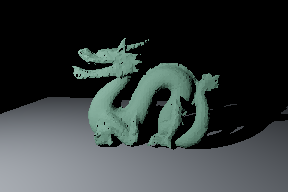
\includegraphics[width=\linewidth]{figures/dragon-direct.png}\\[-1pt]
{\small 点光源照出的龙与投影}
\end{minipage}\hfill
\begin{minipage}{.48\linewidth}\centering
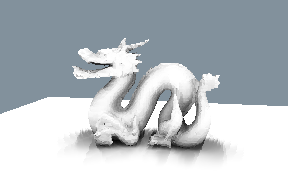
\includegraphics[width=\linewidth]{figures/dragon-visibility.png}\\[-1pt]
{\small GTAO 可见度，白色为 1，黑色为 0}
\end{minipage}\\[4pt]
{\footnotesize\color{quiet}Stanford Dragon，Redflag Vulkan，同一机位的 $288\times192$ 输出。蓝灰色区域没有模型。}
\end{center}

相机看向龙爪边的地面，深度图只记录每个像素最先看到的表面。LearnOpenGL 的 SSAO 教程在这一点周围取样，对照深度图估计有多少处被遮住。GTAO 仍然用到这些表面，但会沿几个方向分别寻找遮挡物的轮廓。想象用一张竖纸同时切过相机和地板上的点，龙爪便在纸上留下一条轮廓线。把这张纸绕观察方向转几次，每次找到轮廓的最高处，就能估计表面总共还能看到多大一片天空。

% 公式推导
沿刚才的纸面来看这小块地板。取从地板指向相机的单位方向 $v$，截面上与 $v$ 垂直的单位向量 $t$。纸面上任一入射方向可写成 $\omega=v\cos u+t\sin u$，其中 $u$ 从相机方向开始量。法线 $n$ 受光的余弦是 $n\cdot\omega$，球面上这段圆弧对应的面积还含 $\sin u$。可见弧从 $0$ 延伸到遮挡角 $h$，也要在法线所在半球的边缘停下。找到遮挡轮廓后，剩下这段积分就能直接算出。

% 公式
设 $a=n\cdot v,\ b=n\cdot t$，单侧截面的照明贡献为
\[
  I(h)=\int_0^h(a\cos u+b\sin u)\sin u\,du
      =\frac{a}{2}\sin^2 h+b\left(\frac h2-\frac{\sin(2h)}4\right).
\]
若地板正对观察者，$a=1,b=0$。无遮挡时 $h=\pi/2$，每侧贡献 0.5，两侧正好得到一整份可见度。$h$ 降到 $\pi/4$，这一侧贡献就降到 0.25。这个例子能检查半球归一化的系数。
\clearpage
% 逐行伪代码
\subsection{在深度图上寻找遮挡}
\noindent{\small\color{quiet}按 GLSL 整理的伪代码\quad\href{run:../../Redflag/src/Redflag/Renderer/ScreenSpace/Shaders/GTAO.comp}{\texttt{GTAO.comp}}}\par\nopagebreak
\begin{lstlisting}[escapeinside={(*@}{@*)}]
blocked = 0
for slice in fourDirectionsAtThisPixel:
    for side in [left, right]:
        h = angleWhereThisSideLeavesNormalHemisphere()
        for distance in eightDistancesWithinRadius:
            neighbor = nearestSurfaceAt(project(point + tangent * distance))
            if neighbor is above the surface and inside radius:
                next = angleBetween(view, neighbor - point)
                if next < h:
                    (*@{\footnotesize\color{quiet}只扣掉两条轮廓之间新增的那段遮挡。}@*)
                    blocked += (I(h) - I(next)) * weight(length(neighbor-point))
                    h = next
visibility = clamp(1 - blocked / 4, 0, 1)
\end{lstlisting}
箱子前面的地面向四周收光。在同一截面上，近处箱沿已经遮住一段圆弧，远处柱子可能挡住另一段。半径为 $r$ 时，前 $0.6r$ 内的样点保留全部遮挡，之后用平滑曲线减弱，到 $r$ 时权重为零。每次只给新挡住的那段弧乘距离权重。如果让远处的样点把整条轮廓一起淡出，紧贴箱壁的地面也容易过亮。

默认 $r=0.65$ 个场景单位，按米建模时就是 65 厘米。一个像素量四个截面，每侧查看八个位置。四个相邻像素稍微转动各自的截面，合在一起能量到十六个方向。\texttt{GTAOFilter.comp} 在周围 $3\times3$ 个像素里按离中心的远近取平均。箱壁和地面的法线相差约 $90^\circ$，两边各自取平均，柱脚的边缘便能留下来。最后再应用面板里的遮蔽强度，将结果乘到环境光上。

% 接口与数据结构
\begin{fields}
\texttt{GISurface} & 可见表面的世界位置、法线和底色。当前实现直接读世界位置，省去从深度图还原位置的一步。\\
\texttt{AORadius} & 世界单位。半径越大越能看到远处遮挡物，固定八步也会变得更稀。\\
\texttt{AOIntensity} & 对可见度施加指数。输出第四通道保留遮蔽系数，可把它只乘在间接漫反射上。\\
\end{fields}

在 Sponza 将半径缩到 0.0001，旧版固定方向采样的平均可见度从 \measured{ao_mean} 变为 \measured{ao_negligible_radius_mean}。镜头外的柱子无法出现在这份表面图里，也不能投下屏幕空间遮蔽。移动相机的实测和局部放大图见《渲染性能实测》的“移动相机下的柱脚遮蔽”。

可见弧积分见 Jimenez 等人的技术报告第 2 节。Intel 的 XeGTAO 实现说明也介绍了半球射线参考与邻域过滤。
